\chapter{Produktstruktur}\label{ch:produktstruktur}
Der Produktstrukturplan ist eine grafische Darstellung der Struktur unseres Produktes und ist wichtig
zur Aufteilung des Produkts in seine einzelnen Bestandteile und Teilkomponenten.
Sobald initial die Struktur des Produktes festgelegt wird, kann auf dieser Basis der Aufwand für jede Teilkomponente des
Produkts geschätzt werden, wodurch summiert der Gesamtaufwand für das Projekt berechnet wird. 
Zusätzlich können betroffene Elemente in das Risikoregister eingetragen werden, falls bei Besprechungen innerhalb des 
Teams Bedenken aufkommen bezüglich der benötigten Zeit für die Umsetzung.
Außerdem kann der Produktstrukturplan Grundlage sein für die Ermittlung der Qualitätskriterien für die einzelnen 
Teilkomponenten des Produkts. 
In Abbildung ~\ref{fig:produktstrukturplan} ist der Produktstrukturplan für unser Projekt dargestellt.
\vspace{1cm}
\begin{figure}[h]
    \centering
    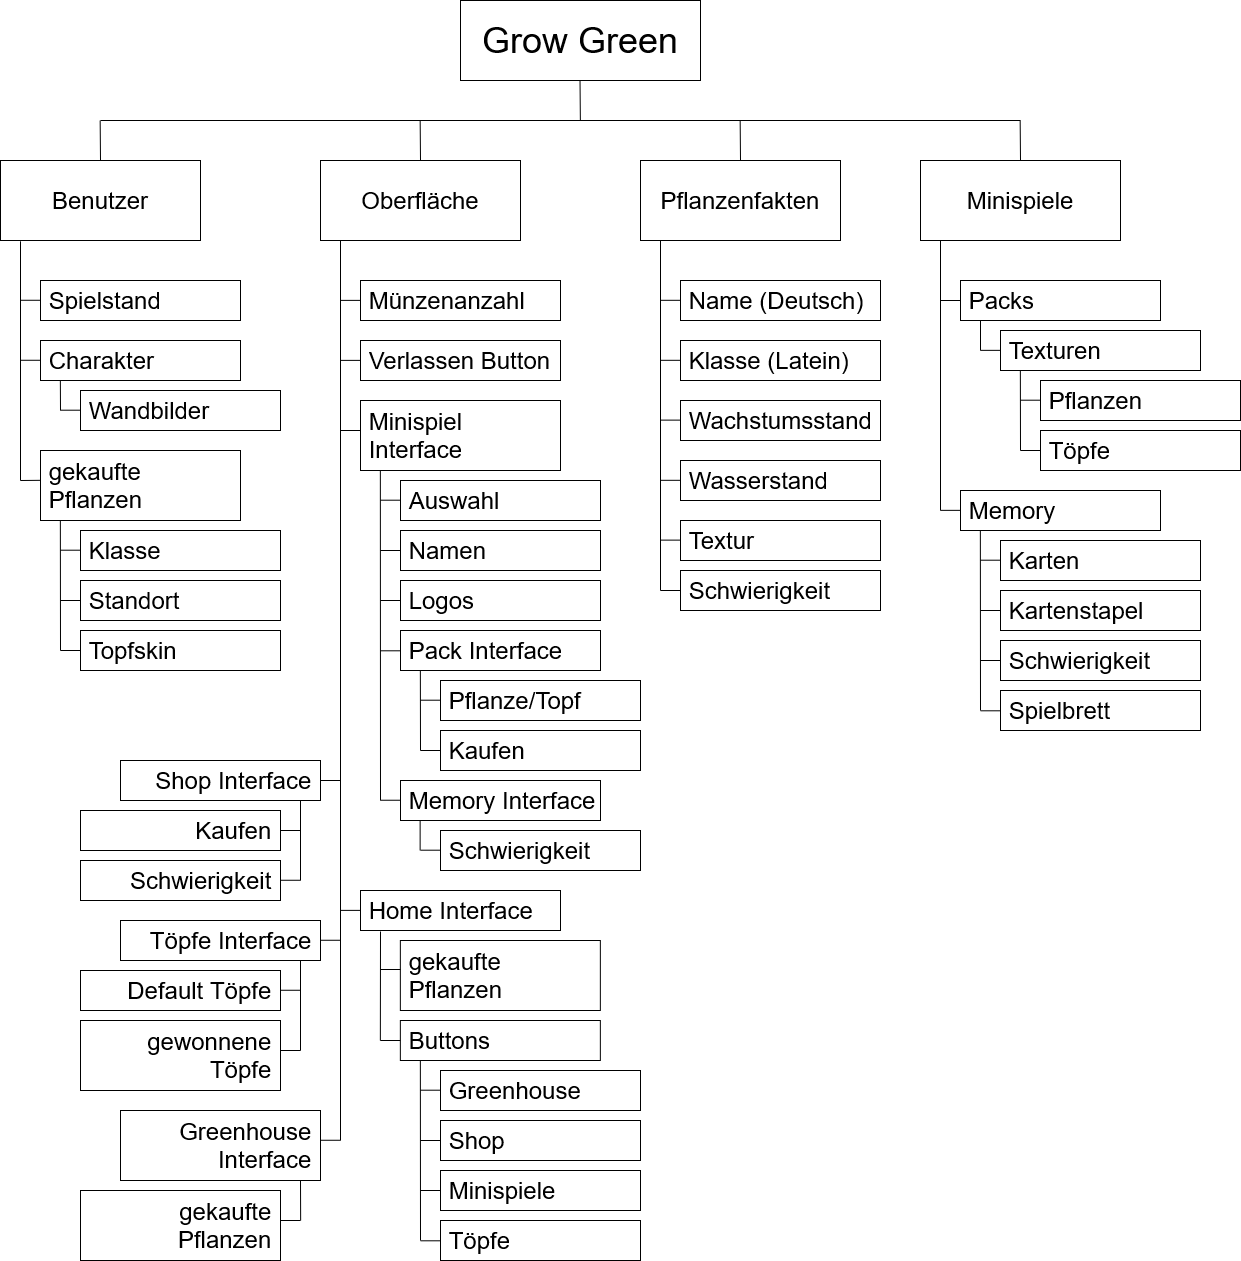
\includegraphics[width=0.8\linewidth]{../bilder/Produktstrukturplan}
    \vspace{0.5cm}
    \caption{Produktstrukturplan}
    \label{fig:produktstrukturplan}
\end{figure}